
\section{Preemptive overview}
In this chapter we face the challenges of reaching a good compromise between stereo augmented reality and immersive VR in one application. To every issue early mentioned in the introduction, one by one, it will be presented an answer in the following paragraphs. More in detail:
\begin{itemize}
\item gear selection and stereo rig design (high field of view and high resolution requirements);
\item image mapping and stereo augmented reality (minimum distortion and facing real and virtual discrepancy in stereo);
\item latency compensation (other discrepancies induced by technical and physical limitations);
\item implementation (all the above with considerations on performance).
\end{itemize}
Will follow in next chapter observation of work's results that could be achieved with the chosen starting gear and deducing possible future developments in the conclusions.

\section{Gear selection}
We preferred to mention first the choices in hardware and software involved in the development of the project; this way we will be able to address the problems one by one and in parallel use our configuration as a practical example. We chose products available to the public that fits best our requirements within reasonable budgets. Software libraries involved focus on simplicity, future integration and come in part as a consequence of some of chosen assets. The table in [figure N] matches hardware/software used with the project goals anticipated so far.

\begin{table}[]
\centering
\begin{tabular}{llll}
\hline
Gear type                       & Model                                & Goals coverage                                                                                                & Limitations                                                                                            \\ \hline
\multicolumn{1}{|l|}{HMD}       & \multicolumn{1}{l|}{Oculus Rift DK2} & \multicolumn{1}{p{0.4\linewidth}|}{
- Low latency \newline
- High refresh rate (up to 75Hz) \newline
- High FOV (up to 110 degrees on horizontal)\newline
- Head pose tracking
}                                                & \multicolumn{1}{p{0.2\linewidth}|}{No documentation on how VR stereo is performed on the eyes}                        \\ \hline
\multicolumn{1}{|l|}{Stereo Rig}    & \multicolumn{1}{l|}{2x Logitech C920}   & \multicolumn{1}{p{0.4\linewidth}|}{
- High framerate (30fps)\newline
- FullHD resolution (1920x1080)
}                                            & \multicolumn{1}{p{0.2\linewidth}|}{Usb2.0 limits bandwidth, frames must be decoded from h.264}                        \\ \hline
\multicolumn{1}{|p{0.1\linewidth}|}{Computer Vision library}    & \multicolumn{1}{l|}{OpenCV 2.4.9}    & \multicolumn{1}{p{0.4\linewidth}|}{
- Camera calibration \newline
- Image undistortion \newline
- Stereo vision \newline
- Performance optimization (CUDA and TBB support)
} & \multicolumn{1}{p{0.2\linewidth}|}{Still a CPU-bound vision library, only partial CUDA support}                                                  \\ \hline
\multicolumn{1}{|l|}{3D Engine} & \multicolumn{1}{l|}{Ogre3D 1.9}      & \multicolumn{1}{p{0.4\linewidth}|}{
- Portability \newline
- Access to rendering pipeline code (open source) \newline
- Shading support \newline
- Compatibility with ROS
}   & \multicolumn{1}{p{0.2\linewidth}|}{Lacks of dedicated development and debug environment (not a technical limitation)} \\ \hline
\end{tabular}
\caption{Hardware and software tools chosen for the experiments.}
\label{gear_table}
\end{table}

The step by step followed for design is:
\begin{itemize}
\item identify class of HMD to build (type of components and its limits);
\item choose lens/mirrors according to focus and FOV to achieve, with acceptable or minimal distortion;
\item choose screen/projector basing on luminosity/contrast and resolution to provide enough detailed images given those lens/mirrors and with a target refresh rate;
\item choose camera (if involved for AR) so that image is closest match for previously defined focus, FOV and resolution;
\item consider additional or replacement lenses to cover needed FOV;
\item account for correcting camera lens distortion (necessary for detection, otherwise not needed if not noticeable by the user);
\item account for blending real and virtual image;
\item account for HMD lens/mirrors distortion (if not noticeable by the user).
\end{itemize}

\iffalse
\subsection{HMD and head tracking}

\subsection{Camera for stereo}
low cost
best resolution/fps rate

\subsection{3D Engine for VR environment}
OculusSDK
Ogre3D

\subsection{Libraries for CV and AR}
OpenCV + tbb + cuda
arUco
\fi

\section{Stereo Rig design}
Assumption is that the two cameras have same technical characteristics and no distortion (or were previously calibrated). According to Paul Burke [24], a good rule of thumb for building up stereoscopic camera rig is to choose camera aperture and focal length first, depending on the the distance from the lens we decide to be on focus. Supposing we have a planar display, it is convenient to keep the zero-parallax plane at the same distance from the viewer, so that convergence and accommodation will keep coherent when watching the part of the scene on focus; this implies that to get convergence right with a parallel setup, one could shift the cameras, the lenses or later the image on the screen, with all the consequences we already discussed. In the case of a toed-in setup, convergence is immediately defined by their tilting angle, with no need for subsequent image trim but at the cost of keystoning.

One great advantage in using a HMD with higher FOV than the cameras is that it is not really a problem to translate the image: once each camera's FOV is correctly mapped into user's view plane, each frame can be shifted or scaled without subsequent loss of FOV. This allows to dynamically adjust convergence after capture, for any stereo rig configuration. Moreover, the nature of 3D environment gives us the ability to easily correct keystoning, by either rotating or scaling the plane image it is projected into, instead of applying such transformation on the image [25]. The main reason left to favour a toed-in over a parallel setup for video see-through in high FOV HMD is the limits of the area covered by the intersection of the frustrums of each camera. If we plan to get stereoscopic effect on objects very close to the user, those objects also must fall in both frustrums. Excluding the more complex off-axis setup, this is only feasible in a parallel setup by raising cameras' FOV, which means switching lenses and introducing higher distortion, or manually tilting them inwards.

\begin{figure} 
\centering   
\begin{minipage}[t]{0.49\textwidth}
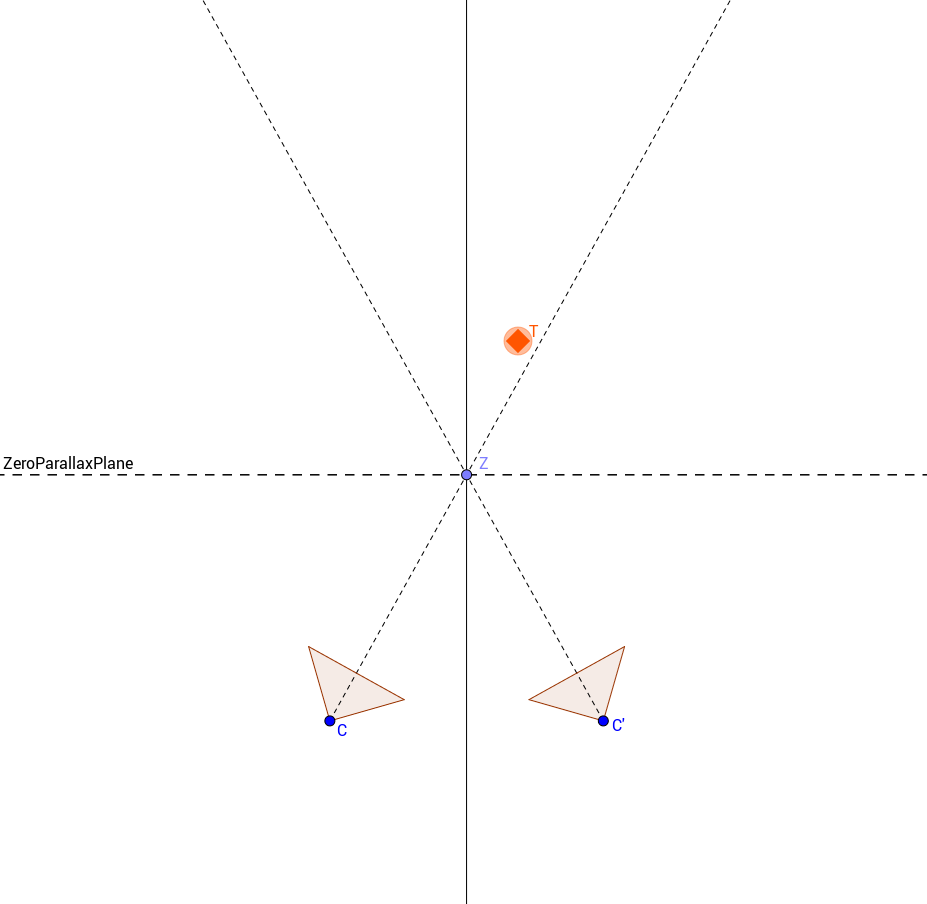
\includegraphics[width=\linewidth, height=7.4cm]{schemas/stereocam_only}
\end{minipage}
%\hspace{\fill}
\begin{minipage}[t]{0.49\textwidth}
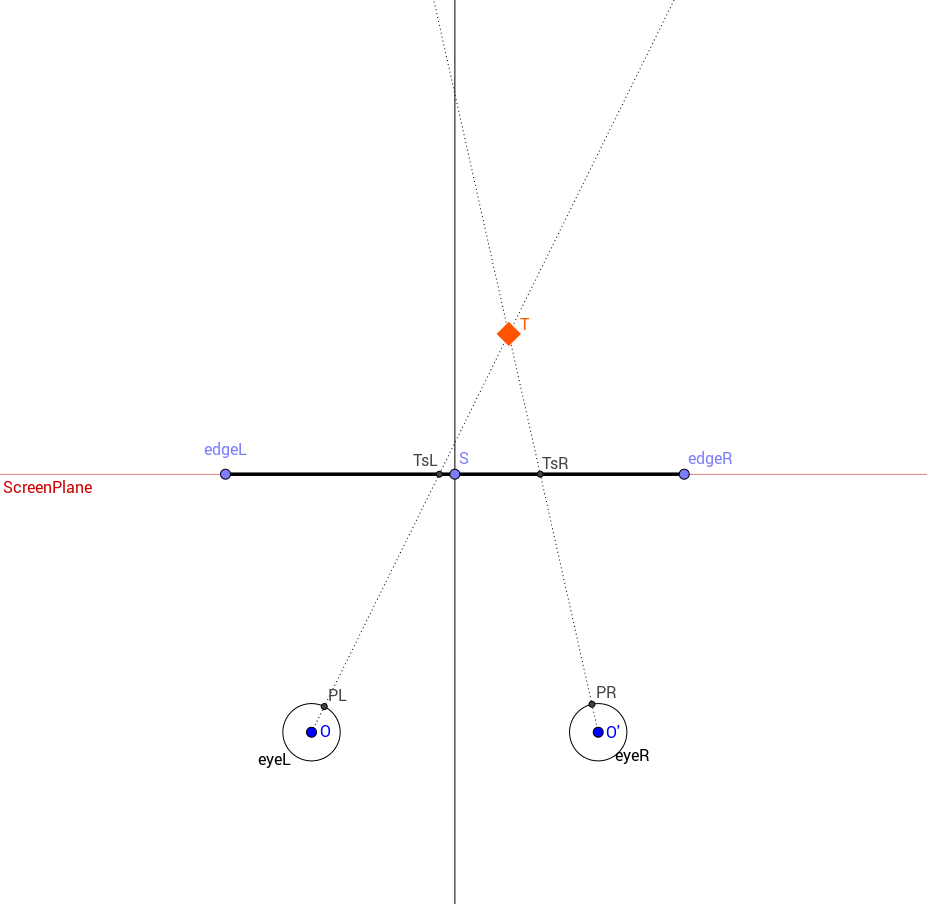
\includegraphics[width=\linewidth, height=7.4cm]{schemas/eyes_only}
\end{minipage}
%\vspace*{2mm}
\caption{Having a stereo camera rig in toe-in configuration (left) has the effect to reproduce the exact depth distance of a target T on a screen (right) where eye-to-eye (OO') and eye-to-screen distances match inter-camera (CC') and zero-parallax distance. Note that the schema ignores keystoning effect, so the geometry is for all stereo configurations where zero-parallax plane is not at infinite}
\label{fig:stereo_eye_camera_comparison}
\end{figure}

Another common norm for stereo video footage is to use 1/30 of the zero-parallax distance as a measure for camera separation [26]. In first-person gaming, one commonly used strategy is to use the height of the camera from the virtual ground as zero-parallax distance and then calculate suggested separation: the result is a rough approximation of the proportions we have in real life. In our case, however, we prefer to keep camera separation as close to IPD: we want cameras to act as user's eyes and images to be perceived as close as reality in manipulation tasks; we will see how this choice will be fundamental for real-virtual matching in later paragraphs. While for footage on a screen the zero-parallax distance can be chosen so that we have the desired depth effect, in our case we will have to match that perceived distance with the virtual world, which will have its own stereo setup.

As for stereo computer vision analysis, stereo calibration can be performed and algorithms can run independently from how images will be displayed to the user. It is anyhow a crucial point to examine in depth how displayed image and the information extracted from it are kept consistent in the 3D environment and in which way they can interact. Assuming we perform detection and place a virtual object in the VR scene accordingly, how can we guarantee that it will be overlapped to the image in the right spot at all times?

The ideal case would be having both virtual and real stereo rigs in off-axis configuration, having real cameras coincident with real pupils. Proposed setup uses off-axis configuration for virtual rig, as also suggested by Oculus documentation and provided by SDK, and toe-in and parallel for the physical rig; in the specific, for standard and wide-angle type lenses (modeled with pinhole model) cameras are toed-in, for fish-eye type lenses instead they are parallel. We will express the reasons for this choice in the following paragraphs.

To keep each camera closest to each eye and minimize virtual sickness [27], constraints implied for the physical cameras are:
\begin{itemize}
\item keeping them at IPD distance (average human reference is 0.064m);
\item placing rig at minimum distance from the eyes allowed by the HMD.
\end{itemize}
The configuration chosen to conduct our experiments is with cameras placed directly in front of user's eyes.

\subsection{Wide-angle lens configuration}
Wide-angle lenses, even with high distortion, still obey to pin-hole camera model. Horizontal FOV for such lenses may vary from 45-50 to 90 degrees with lens distortion increasing ad the edges. This category can partially or completely cover horizontal FOV of a video HMD. One more problem is that these devices declare a vertical FOV that is valid only when the whole sensor surface is used. This is always the case when capturing one single image: it will be memorized in camera buffer and then transmitted to whatever machine requiring it, in an offline fashion. When requiring a constant stream of high definition images, however, device meets buffering, encoding and transmission speed limitations. For instance, our model is a high end consumer usb 2.0 webcam offering up to 1920x1080 (16:9) resolution at a stable 30 fps stream; to achieve this result, our camera not only uses a fraction of the sensor (actual sensor is a 2304x1536 (4:3) so it uses the widest subset of pixels forming a 16:9 image for live capture), but also downscales and encodes in h264 captured frames. Similar performances in usb 3.0 devices leads to much higher cost for industrial applications [28,29].

\begin{figure}
\centering
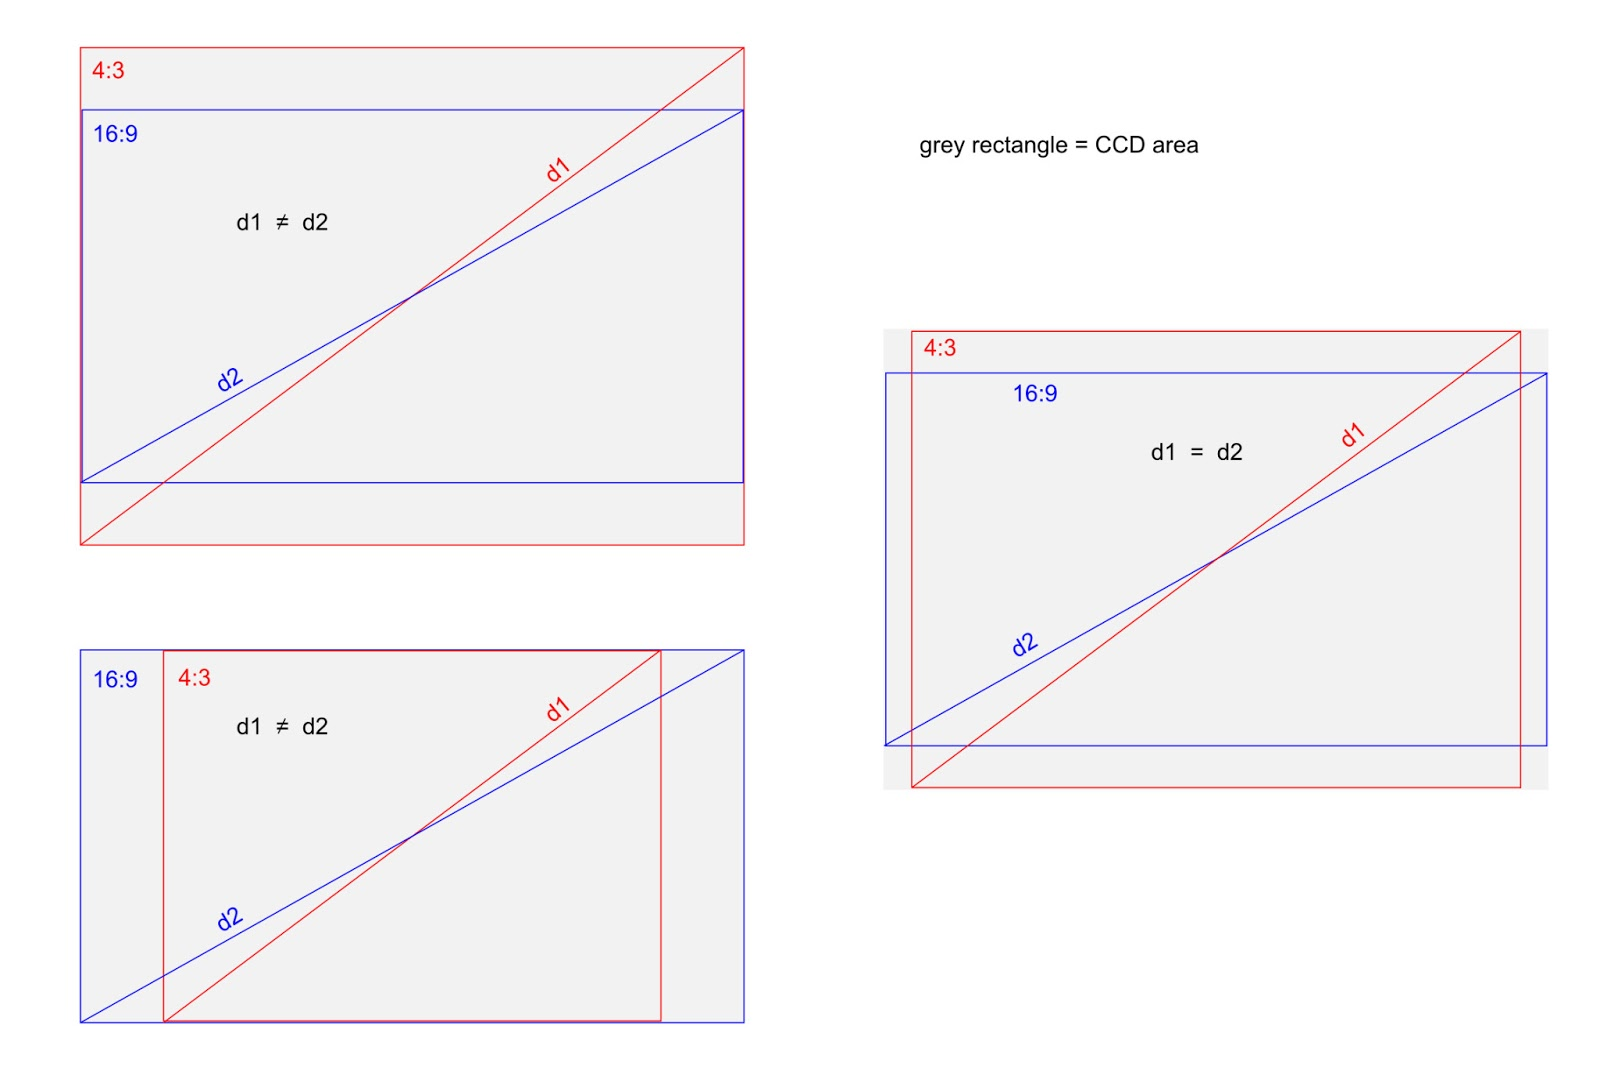
\includegraphics[width=\linewidth]{schemas/diagonal_FOV}
\caption{An overview on how a 16:9 image is extrapolated from a 4:3 sensor and vice-versa (left). Retailers often do not specify which ratio the declared diagonal FOV corresponds to, even though there is always a discrepancy on the vertical and horizontal (right). (source: \href{http://therandomlab.blogspot.se/2013/03/logitech-c920-and-c910-fields-of-view.html}{http://therandomlab.blogspot.se})}
\label{fig:timewarp_timeline}
\end{figure}

Such frame displayed in front of one eye in the rift covers most of its horizontal range, but only about a half of vertical. A solution to this problem has been proposed by William Steptoe [30]: first match per-eye resolution of the HMD with the sensor's, then replace current lens with one with smaller focal length. This implies rotating each camera by 90 degrees, so that the new 9:16 configuration matches closely Oculus Rift DK2 per eye resolution of 960x1080. This is true, although lenses allowing to match camera vertical FOV with Oculus horizontal are very hard to find and would introduce too high distortion and information loss at the edges; it gets indeed coverage of DK1 vertical FOV but was it does not exploit all its horizontal capabilities (figure). Furthermore, there are two major reasons why we chose to stick with horizontal cameras:
\begin{itemize}
\item even assuming possible to cover eye horizontal angles with rotated sensor, there would be a substantial image loss on the vertical, since camera horizontal FOV would have reached much more than needed angle;
\item it is more likely to the user to rotate his head and eyes to the right and left; with non-rotated sensor, stock lens is enough to cover each eye's horizontal, while an enhanced lens can improve vertical coverage and the portion of horizontal out of the border is still useful information that can cope with capture-display latency (discussed in later paragraphs);
\item stock lens provides an efficient mechanism of auto-focus that comes in handy with up-close real object observation; note that focus of each camera is set by default at infinite: due to the short focal length typical of webcams (that usually require high field of view) everything further than N meters is on focus. For closer objects, autofocus can be activated, but both focal length values must keep in sync so that there is no discrepancy in blurriness between the two images.
\end{itemize}
In such limited FOV conditions we opted for horizontal cameras in toe-in configuration. Cameras converge at 40cm from the user, which is our estimated average for basic hand manipulation so tasks. Stereopsis can be achieved for very close objects up to N cm from the user in negative parallax. Instead of a tunnel-like view effect for FOVs insufficiently high in respect to human eye, we get more a window-like view: HMD provides a view range wide enough for user's eyes, but camera image boundaries are visible, implying that real objects are perceived as coming in or out a "window", whose distance corresponds to the zero-parallax. Arms in view closer than this distance are seen as "cropped out" from the bottom, which clearly shows negative parallax limits. Ideally, this window should be moved as close as possible to the eyes (shouldn't be the HMD itself the supposed "window"?) but this is not really practical nor suggested for all the issues discussed above. Note that this fictional plane is only an optical perception: the distance at which the actual virtual object onto which image is projected can be arbitrarily and dynamically changed. This won't matter where real objects will be perceived, but where virtual object will be clipped by such plane. One advantage is the chance to decide whether the image should appear in front or behind static objects in the scene (such as virtual floors and walls) by changing its distance (manually or automatically) in respect to the z-value of such objects instead of acting on the render order.

\iffalse
TOED-IN
(-) edge violation, "see through a window" effect (lower immersion)
(-) keystoning effect at edges, but reducible
(+) compensate the low stereo cues area of parallel config
(+) easy to implement
(+) good vertical disparities (VSR)
\fi

\subsection{Fish-eye lens configuration}
Way more high FOV can be gathered by fish-eye lenses, which can cover angles from 120 to 170 degrees, up to 190 in extreme conditions. Inevitably, lens distortion is also very high, but responds to a different camera model, where there is no unique optical axis, but infinite spanning from lens focal center to every point of its spherical surface [31]. This is way image captured from a planar sensor from a fish-eye lens model appears as a circle, with almost no distortion at its center, compressing toward the edge until disappearing on the boundary: this is what we get when projecting a spherical surface on a plane. This is addressed as epipolar or stereographic projection in geometry and is widely used in fields like geography and cartography [32] where the need to map targets non-planar by nature into planar representations is met.

For computer vision, but also for a naked eye, such images need to be undistorted to see the scene in the proper way. On a 2D plane, by undistortion we intend a sequence of transformations or re-projections that returns, in the end, a 2D picture. For what we said about the capabilities of a fish-eye lens, this shows a clear limit: it requires a planar surface of infinite dimensions to reproduce 180 degrees of FOV correctly, and still impractical proportions for values as high as the human eye's.

(figure)

Our solution borrows the techniques used in immersive environment based upon hemispherical domes [33]. In particular, how omnidirectional images can be displayed so that the combination of viewer position and display itself perform the undistortion we are looking for: in principles, reverting a stereographic projection from the plane, the result of fish-eye lens capture on the planar sensor, to its original 3D representation. Since we have two capture devices, what we also need is a stereo configuration to achieve stereopsis with such image pairs. Supposing we have a viewer in the center of a physical semi-spherical dome, capable of stereo, with eyes looking straight at its middle; the simplest configuration would be rotating each image, meant for each eye,  virtually inwards such that zero parallax occurs at the correct distance along view direction and project them to the same surface [34]. This can correspond to our setup with toed-in cameras and fish-eye lenses, where images are live captured and "virtual" rotation of the image corresponds to a real rotation of the sensors. But as Paul Bourke stresses, correct parallax information is returned by the sistem only when viewer's eyes are oriented straight forward, towards the region where considerations made for pinhole toed-in stereo apply. The alternative to this approach is called off-axis fish-eye projection [35] which can be considered the counterpart of image displacement in planar displays: each omnidirectional image is virtually shifted and then reprojected on the dome, so that satisfactory depth sensation is formed for viewing directions different from the one mentioned above. Our camera setup can easily match this dome projection algorithm by shifting them perpendicularly to viewing direction, in a parallel configuration, which is our chosen option for capture FOV higher than what is allowed per-eye by the HMD.\\
For our experimental setup, we can take advantage of the virtual 3D environment to recreate the same conditions: a half sphere mesh, solidal with user's virtual head,  can be used as a dome by orienting face normals towards the center and using the raw fish-eye image as a texture. To avoid complex shading algorithms, a pre-compiled UV map has been used and the chosen equipolar mapping method is shown in figure N.\\
Note how this solution fits elegantly to solve most of the problems encountered so far:
\begin{itemize}
\item in both omnidirectional off-axis and toe-in approach, viewer experiences a decrease in parallax information towards the edges of the dome (angles next to -90 and +90 in respect to its original view direction); this loss can only be appreciated in a real dome, where an individual can actually rotate his head in respect to it, meanwhile in our setup he is only able to rotate his eyes, which in turn cannot get disparity on its sight borders by nature; such extreme eye movement are also unlikely to happen in reality;
\item HMD allows us to return to each eye its own view, meaning a different dome and projected image; therefore both virtual eyes can be placed at the center of the semi-sphere at all times, an ideal and never verified condition for physical stereo dome environments;
\item the symmetric nature of the projection and its extended FOV can come in handy for compensating latency issued between image capture and head movement without the user noticing, as we will discuss in later paragraphs.
\end{itemize}

\iffalse
PARALLEL with high fov
(+) no edge violation (close objects are welcome, high immersion)
(+) no keystoning
(+) no need to toe-in to compensate low fov..
(-) .. but still can be very distorted at edge (need high quality lens!)
(-) no stereo cues at the edge of the image
(-) hard to implement (due to additional undistortion)
(+) good vertical disparities (VSR)
\fi

%\section{Application pipeline}


\section{Image mapping}
As AR interaction scene is finally rendered on a screen, a straightforward approach could be to first render the background or the skybox, then render correctly FOV mapped image and display it, then render virtual objects on top. This approach is what happens for AR applications displayed on a common display, where the actual background is the real image in all conditions. On a video HMD, however, the parameters according which image is finally shown to the user can be much more complex than screen dimensions and resolution: mirrors or other optical solutions are involved to cover the needed FOV, meaning that the image on the screen must cope with introduced distortions, much like what Oculus Rift does. The mapping between HMD and the screen and the system implementing it is device-dependent: such information can be gathered only from documentation or from SDK. Moreover, any further adjustment on the image must be carefully implemented by tweaking the projection formula used, which can be not very intuitive and error prone when editing it in code. When working with a 3D engine, where z-buffer and rendering is usually hidden, the real image overlay step must be implemented specifically for that developing environment.\\
Our approach proposes a solution to manage the 2D image FOV mapping and re-projection on video HMD independent from its physical implementation: if the HMD is capable of rendering properly a 3D scene, then is also capable of blending a 2D camera image in it, whatever the FOV discrepancy.

\subsection{Pinhole camera model mapping}
In a 3D virtual environment, scene is rendered through a virtual camera, modelled by a view and perspective matrix: the first responsible for transforming vertices coordinates from world to camera reference, the latter used for the actual 3D to 2D projection. For what it does, the latter is cousin of the intrinsic parameters matrix used in computer vision, but still differs in the form.\\
Hartley and Zisserman's intrinsic matrix [?] is parametrized as
\begin{equation}
	K = \left ( 
    		\begin{array}{ c c c}
    		f_x & s   & x_0 \\
    		0  & f_y & y_0 \\
    		0  & 0   & 1 \\
    		\end{array}
    \right )
\label{hz_intrinsic_matrix_original}
\end{equation}
being $f_{x}$ and $f_{y}$ the horizontal and vertical focal lengths and $x_{0}$ $y_{0}$ the principal focal point offsets. The former determines the range of angles FOV covers while the latter decides the skew of the optical axis that may represent, for instance, shift of the sensor or the lens (done on purpose for off-axis configurations). We will not consider the skew $s$, which would describe a relative tilt of sensor in respect to the lens or vice-versa, as it is not of interest in our work.

Projection operation is performed in computer graphics by the "projection matrix", documented as \ref{gl_proj_matrix_original}. Two conceptually different operations are performed:
\begin{itemize}
\item actual perspective projection (from 3D to 2D points);
\item conversion into normalized device coordinates (NDC) which is an implementation dependency of the rendering pipeline.
\end{itemize}
\begin{equation}
P = \left( \begin{array}{cccc} \frac{2 near}{right - left} & 0 & A & 0 \\ 0 & \frac{2 near}{top - bottom} & B & 0 \\ 0 & 0 & C & D \\ 0 & 0 & -1 & 0 \end{array} \right)
\label{gl_proj_matrix_original}
\end{equation}
where
\begin{equation}
\begin{array}{c}
A = \frac{right + left}{right - left} \\[0.6em]
B = \frac{top + bottom}{top - bottom} \\[0.6em]
C = -\frac{far + near}{far - near}  \\[0.6em]
D = -\frac{2 \; far \; near}{far - near}
\label{gl_proj_matrix_original_details}
\end{array}
\end{equation}
Note that the virtual reproduced FOV is expressed in terms of $right$, $left$, $top$, $bottom$ edges of a virtual image plane, which will result in the rendered frame. Also both projection matrix use a reference system that only differs from z-axis direction (Figure N).

\begin{figure} 
\centering   
\begin{minipage}[t]{0.45\textwidth}
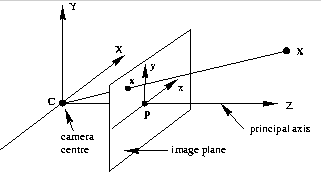
\includegraphics[width=\linewidth, height=4.4cm]{schemas/hz_camera}
\end{minipage}
%\hspace{\fill}
\begin{minipage}[t]{0.45\textwidth}
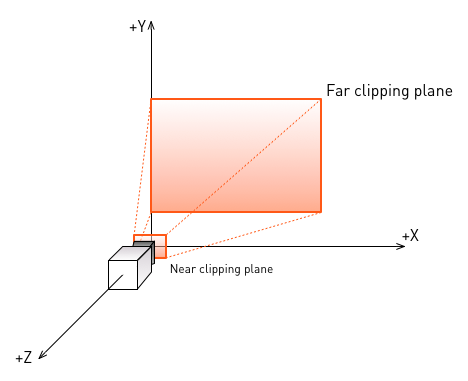
\includegraphics[width=\linewidth, height=4.4cm]{schemas/gl_camera}
\end{minipage}
%\vspace*{2mm}
\caption{Pinhole camera model (left) and GL camera model (right) "looking" at opposite directions.}
\label{fig:stereo_eye_camera_comparison}
\end{figure}

Following the steps of Kyle Simek's work[?], intrinsic matrix (\ref{hz_intrinsic_matrix_original}) reference system can be then inverted on Z axis (by inverting sign of 3rd column) and can include additional z-depth information to match closer $P$ from \ref{gl_proj_matrix_original} closer:
\begin{equation}
K_{persp} = \left( \begin{array}{cccc} f_x & s & -x_0 & 0 \\ 0 & f_y & -y_0 & 0 \\ 0 & 0 & X & Y \\ 0 & 0 & -1 & 0 \end{array} \right)
\label{hz_intrinsic_matrix_extended}
\end{equation}
where
\begin{equation}
\begin{array}{c}
X = near + far \\
Y = near * far
\end{array}
\label{hz_intrinsic_matrix_extended_details}
\end{equation}
By introducing in \ref{gl_proj_matrix_original} focal lengths different than $near$ by altering scale of virtual image plane
\begin{equation}
\begin{array}{c}
left' = (\frac{near}{\alpha}) left \\
right' = (\frac{near}{\alpha}) right \\
top' = (\frac{near}{\beta}) top \\
bottom' = (\frac{near}{\beta}) bottom
\end{array}
\label{near_alter_scale}
\end{equation}
and non-zero principal point offset by further translation of frame boundaries
\begin{equation}
\begin{array}{c}
left'' = left' - x_0 \\
right'' = right' - x_0 \\
top'' = top' - y_0 \\
bottom'' = bottom' - y_0
\end{array}
\label{near_alter_offset}
\end{equation}
we can simulate a general intrinsic camera matrix with zero skew $s$.

At this point, relevant camera characteristic parameters can be extracted from both matrices. The main difference lays in the model: "Normally, the film plane of a (real) camera is behind the focal point (i.e. the aperture) of the camera. The image can, however, be regarded as lying on a virtual image plane in front of the focal point. This arrangement is essentially the same as the virtual camera setup used in computer graphics rendering: the focal point is the "eye" point, the size and position of the image rectangle controls the field of view, and the perpendicular to the virtual image plane provides the "gaze" direction" [36]. This means that any HMD (or any other device displaying virtual imagery from 3D world) will most likely be using a virtual camera much like a real one; we say "most likely" because there do exist other less diffused proposed models for 3D rendering applications, such as Vrui [37].\\
Rethinking real camera in terms of image plane, we can port its FOV and image into the virtual camera with a planar mesh in front of it, perpendicular to its view vector, where size and distance from the virtual camera focal point are strictly correlated.

Consider its horizontal dimension $H_{dim}$ and its distance $d$ from the center of projection, so that it covers $H_{fov}$ of FOV angle; being
\begin{equation}
\alpha = \frac {H_{fov}} {2}
\end{equation}
by trigonometric construction we have
\begin{equation}
\tan \alpha = \frac {H_{dim}} {2 d}
\label{Hdim_relation}
\end{equation}
Consider now the relationship [n?] between horizontal FOV $H_{fov}$ of a pin-hole camera and its relationship with horizontal sensor dimension $s_{w}$ and focal lenght $f_x$: 
\begin{equation}
H_{fov} = 2 \arctan \frac {s_{w}} {2 f_x}
\label{Hfov_relation}
\end{equation}
By combining the \ref{Hdim_relation} with \ref{Hfov_relation}, we have 
\begin{equation}
H_{dim} = \frac {s_{w} d} {f_x}
\label{fov_distance_relation}
\end{equation}
The same can be verified with vertical counterparts $V_{dim}$, $s_{h}$ and $f_y$.

In other words, fixing a distance $d$ in \ref{fov_distance_relation} will determine horizontal and vertical size of the rectangle for the known real camera intrinsic parameters, and their ratio keeps constant when varying the distance. In fact, it does not make mathematically sense to define unique values for size and distance: virtual image plane is only an abstraction and can represent any parallel planar slice of the virtual camera frustrum, from distance "epsilon" to "infinite", so the projection can be generated by any of these positions. The reader can then ascertain that, by using a mesh as instance of the real image plane, camera FOV is not dependent from virtual camera FOV. HMD system can establish its own virtual camera parameters and mapping, covering a range of view angles in the virtual world, while real camera will have his own intrinsic camera matrix, with its own set of horizontal and vertical angles: as soon as real and virtual focal points overlap in the 3D scene, no discrepancy can be observed. An interesting observation is that we do not need to work with real unit values: calibration camera result may be expressed in pixels or meters but in the 3D scene they will still be expressed in virtual units (that can have any physical meaning) since all that matters is the ratio between those values.\\
One exception may arise from consistent off-axis configurations: if for either real or virtual camera focal point is off the optical axis, to keep real image plane centred it should be shifted sideways by the distance between the two positions. This happens because our model simplification that only considers distance on the view vector of the camera, ignoring oblique optical axis. Model can be enhanced by extracting focal points coordinates from the matrices and applying the offset to the plane, but since it would be just a slight amount for Oculus Rift virtual cameras and this is the same operation that can be manually performed for convergence adjustment, such exception is not caught in our implementation.

\subsection{Fisheye camera model mapping}
Considerations previously made for fish-eye image projection find direct application in the method proposed for pinhole camera. Instead of using a plane, a half "UV" or "Polyshpere" mesh is used in omnidirectional dome fashion, having its center coincident with focal point of the virtual camera (representing the eye). Distance and size condition is always preserved when varying sphere's scale symmetrically on the three axis (without deforming its original shape) since sphere has its pivot point in the virtual eye and covering 180 degrees in both horizontal and vertical direction.\\
There is a problem however with this setup: while the rectangular plane matches perfectly image to be projected in size, the sphere covers maximum view at all conditions, meaning that fish-eye circle will very unlikely cover the whole surface, unless perfectly matching the FOV. Moreover, the way such image lays on the rectangular camera sensor is totally dependent on how lens is mounted and camera specifications. For this reason, once frame is taken, data must be mapped correctly on the mesh, which in turns means:
\begin{itemize}
\item placing the center of fish-eye circle in front of user's view;
\item scaling the fish-eye circle so that it covers the correct amount of FOV;
\item hiding the part of the image without information (hiding black areas out of the circle).
\end{itemize}
The extraction of the fish-eye circle could be performed by computer vision algorithms, detecting the black areas and determining its center: the latter to be performed at least once, while image cropping should be performed for each captured frame. To determine lens FOV, methods specifically meant for fish-eye image calibration exist and are provided by common use computer vision libraries such as OpenCV [40] and Matlab [41]. Once FOV is known, we can initially assume it to be symmetrical and map fish-eye circle on the dome surface. We will now see how a correct dome display of the image is straightforward with only means of UV map coordinates transformation.\\

Consider the result of a orthogonal stereographic projection of a half-sphere into a plane: it forms a perfect circle, having same diameter as the sphere. Assume now a pre-compiled UV map that implements the correspondence between points of the plane (an image) and the sphere surface (the dome mesh) from such projection. For simplicity, consider its initial center in $C^{map}_{u,v}=(c_x,c_y)=(0,0)$ and its rightmost and topmost boundary in $(1,0)$ and $(0,1)$ respectively, forming a perfect quarter of circumference on a perfectly square image and ray along $u$ and $v$ axes is $r^{map}_{u}=r^{map}_{v}=1$; this choice will help making next calculations more intuitive and independent from previous implementation choices of UV mapping.\\
Having identified the following data:
\begin{itemize}
\item image frame dimensions $w_{px}$,$h_{px}$ (in pixels)
\item fish-eye circle center coordinates in the image frame $C^{fsh}_{x,y}=(c_x,c_y)$ (in pixels)
\item fish-eye circle ray $r^{fsh}_{px}$ (in pixels)
\item fish-eye $fov_{deg}$ (in degrees)
\end{itemize}
we may want first to convert from pixels to UV space. Since $w_{px} \ne h_{px}$, $r^{fsh}_{px}$ will have two different dimensions along $u$ and $v$ axes:
\begin{equation}
\begin{array}{c}
r^{fsh}_{u}=\frac{r^{fsh}_{px}}{w_{px}}\\[0.6em]
r^{fsh}_{v}=\frac{r^{fsh}_{px}}{h_{px}}
\end{array}
\end{equation}
The same goes for $C^{fsh}_{x,y}$, where
\begin{equation}
\begin{array}{c}
C^{fsh}_{u}=\frac{C^{fsh}_{x}}{w_{px}}\\[0.6em]
C^{fsh}_{v}=\frac{C^{fsh}_{y}}{h_{px}}
\end{array}
\end{equation}
Since we chose $r^{map}_{u}=r^{map}_{v}=1$, we can easily rescale UV map points so that UV circle can match fish-eye circle dimension and consequently apply offset so that $C^{map}_{u,v} \equiv C^{fsh}_{u,v}$. In homogeneous coordinates:
\begin{equation}
T_{scale} = \left( \begin{array}{ccc}
r^{fsh}_{u} & 0 & 0 \\[0.5em]
0 & r^{fsh}_{v} & 0 \\[0.5em]
0 & 0 & 1
\end{array} \right)
\qquad
T_{offset} = \left( \begin{array}{ccc}
0 & 0 & C^{fsh}_{u} \\[0.5em]
0 & 0 & C^{fsh}_{v} \\[0.5em]
0 & 0 & 1
\end{array} \right)
\label{UV_scale_offset_180}
\end{equation}
With subsequent application of $T_{scale}$ and $T_{offset}$, the image circle is mapped on the half-sphere so that its surface is perfectly covered. This would be enough for correct mapping only if $fov_{deg} = 180^{\circ}$, which is the maximum coverage allowed by this projection and the dome. Since angle of view and angle on the sphere are proportional, UV scaling factors in \ref{UV_scale_offset_180} can be further reduced by the actual $fov_{deg}$ factor
\begin{equation}
\begin{array}{c}
r'^{fsh}_{u}=\frac{r^{fsh}_{u} \cdot fov_{deg}}{180^{\circ}}\\[0.6em]
r'^{fsh}_{v}=\frac{r^{fsh}_{v} \cdot fov_{deg}}{180^{\circ}}
\end{array}
\end{equation}
Since all the scaling is performed prior to translation, the additional factors can be merged in $T_{scale}$ by replacing the factors in \ref{UV_scale_offset_180} and resulting in a $T'_{scale}$.
As a result
\begin{equation}
\overbrace{
\left(\begin{array}{c}
u'\\
v'\\
1
\end{array}\right)
}^{\widetilde p'_{u,v}}=
\overbrace{
\left( \begin{array}{ccc}
r'^{fsh}_{u} & 0 & C^{fsh}_{u}\\[0.5em]
0 & r'^{fsh}_{v} & C^{fsh}_{v}\\[0.5em]
0 & 0 & 1
\end{array} \right)
}^{T=T'_{scale} \cdot T_{offset}}
 \cdot 
\xoverbrace{
\left(
\begin{array}{c}
u\\
v\\
1
\end{array}
\right)
}^{\widetilde p_{u,v}}
\label{UV_fisheye_map}
\end{equation}
which summerizes the dome fish-eye mapping with the suggested UV map start configuration.

With a generic UV map, getting the same result is trivial. It is sufficient to postpone to \ref{UV_fisheye_map} the necessary translation and scaling that transforms $C^{map}_{u,v} \longrightarrow (0,0)$ and $r^{map}_{u,v} \longrightarrow (1,1)$ so that they are performed in advance. The reader may solve the resulting combined transformation matrix for the generic case, that we prefer to keep separate.

By implementing the transformation as a fragment shader algorithm in sphere material, we have been able to reproduce its results; also by assigning zero alpha value to the area outside the circle (by either targeting black color values or better a binary mask) it is no longer necessary to preemptively crop each frame from the black area since such operation is a direct consequence of UV mapping.\\
In our application, fish-eye image data extraction has not been implemented and is left for future development. However, by means of the shading algorithm, UV map offset and scale can be tweaked manually at runtime with a direct feedback to the user: such feature allows to display not only real video stream from the cameras, on which we have control for calibration, but also offline stereo omnidirectional imagery captured by unknown fish-eye lenses.

\section{Implementing stereo augmented reality}
A premise of our pipeline design is to be able to perform computer vision or stereo computer vision independently from the method used to finally render images to the user. One may choose to enhance the frames and display such to the user or merely extracting information from one or both cameras leaving their view untouched. While the application unlocks such possibilities, our implementation focuses on coherent display of the two worlds, meaning blending (raw or filtered) real and virtual images and virtual content with real content, alias augmented reality. Technically speaking, real world content in a 3D virtual environment would classify such application as augmented virtuality, as we mentioned in the introduction; however, for this project, our final goal was not focus on VR (whose aspects eventually come in play) but to implement see-through and model an augmented reality headset through it.\\
Reader can agree that with sufficient knowledge in computer vision and shading scripting it is straightforward to alter camera image and render it to output; only limitations are performance and curiosity. The same cannot be said when working with virtual objects partially or entirely generated by information extracted from real images. In most elementary consumer AR applications [4,5], virtual entities are rendered on top of a real image which covers the entire screen, so that the gap between virtual and real is evident only for the limited size of the screen. In our case, image can cover in part or entirely the user's view: anything virtual placed on top of the image must persist in the 3D world he is experiencing, in or out the image. Such objects can be arbitrarily placed in the environment just like a VR-only application or placed somewhere according to what is sensed outside, exactly like position or orientation tracking sensors do to place user's avatar according to its real movements. With the use of cameras, we can take advantage of modern computer vision to experience what is seen by the user when the whole view around him is augmented.\\
Consider for simplicity an ideal camera, with no distortion and intrinsic matrix known, responsible to detect a the marker on the image. Knowing its physical dimension, it is possible to obtain position and orientation of the marker in respect to camera reference system. Such information can be directly used to place a virtual object in the 3D space, once real and virtual reference systems coincide. Given the considerations and the choices in setting up image projection mesh in respect to the virtual camera, there is no further transformation to be done: position and orientation of the real marker are only relative to real camera focal point and its orientation, whose model in turn overlaps with the virtual camera. This implies that by construction the projection of the marker will coincide with virtual object projection, as soon as coordinates of the latter are expressed in the virtual camera coordinate system. This has one relevant advantage: in our stereo rig, whether the marker is detected by the left camera and the entity position/orientation is set accordingly, this will appear also perfectly overlapped in right camera view since the 3D scene is shared between both eyes, as shown in picture (figure N). Stereoscopic perception is achieved by both objects seamlessly.\\
In practice, each frame from a real camera must be undistorted before working with detection algorithms and computer vision in general. After distortion correction, horizontal and vertical FOV and the projection of the focal point on the image plane is computed and put into the intrinsic matrix. Such information is then used to place the virtual projection mesh correctly in the scene, so that the focal point of real and virtual cameras will coincide, as previously said. The undistorted image, however, will be subjected to changes and marker detection (or any other elaboration) will be performed on that result. For a pinhole camera, the resulting image should be then projected in the 3D scene instead of the raw one, unless the distortion is far from noticeable: virtual objects will be correct anyway, but its background has to keep coherent in proportions. In our experiment, cameras presented low distortion at the edges so user could not tell the difference between using raw or rectified image.\\
Using a fish-eye lens is instead a different argument: its pinhole camera equivalent is used to get a rectified result and intrinsic parameters, which is data used by computer vision, while the raw version is used in the 3D environment with its own undistort mechanism. Both return an undistorted view of the camera but it may not be straightforward how the overlap can be guaranteed. Again, all that matters is that focal points correspond and the undistortion is performed correctly in both cases. The computer vision algorithm may not work on the whole original FOV (figure N), but the detected extrinsics will still be expressed in respect to the focal point set in camera intrinsics meanwhile virtual camera can have its set of horizontal and vertical FOV values. Note that while for pinhole model projection mesh can be simply shifted to compensate errors in focal point correspondence, UV map coordinates must be shifted as well to achieve the same result with fish-eye model mesh.\\
Some further considerations must be done for stereo convergence calibration: shifting inwards or outwards the two images (or any other translation) will disrupt such alignment. The previous explained implementation works for toed-in convergence and parallel fish-eye, but will inevitably fail where further convergence adjustments are made in software. In this case, one may want to extend our geometrical model of the virtual stereo rig by putting a constraint on virtual object position and scale, so that it is also slightly shifted and returns to each eye the correct view, even though this can be seen as a "hack" because its final dimensions and coordinates will differ from what was originally perceived by the real cameras.\\
By means of head tracking, we can further improve the perceived detection performance: once an AR marker is first detected, its coordinates can be expressed from original virtual camera to virtual world coordinates and used to position the AR object permanently in the 3D scene; since camera image is in our setup dependent from HMD pose and user's head movements are mapped into virtual world, the correspondence between virtual object and marker will remain valid also when marker is not in view, as soon as marker has not moved. This is extremely useful in applications when there are both complete positional and orientation tracking and marker is not supposed to move [42], but still mitigates failures in detection, caused by motion blur (very likely since cameras are mounted on user's head)  or marker partially in view, and the only head orientation is used, as in our experiment. Virtual object will obey to virtual world physics until it is "synced" again with real world information. Other algorithms in need of such information could be optimized by using coordinates from virtual world which provides at best the real value and at worst a good approximation.

\section{Live capture latency compensation}
So far we presented an approach to reduce the perceptual gap between virtual world and virtualized real world through stereoscopy and VR, while reaching for distortion, resolution and FOV goals. We then implemented an AR example to demonstrate its convenience when dealing with real and virtual objects. Although these results are good from a vision point of view, latency is still a problem we did not tackle.
As mentioned in previous work, Oculus offers the timewarp mechanism as a mitigating solution for system latency between head movement and render, by re-projecting the view right before it is displayed to the eye. As a matter of fact, we have an additional problem of the same sort: the time of capture from each camera will always differ from the time it will be displayed in the scene, meaning we have a discrepancy in response between real and virtual.\\
The difference in frame rate is also a problem. An obvious choice is to choose camera with a capture rate as high as application render rate, but this can be again very expensive; the whole system frame rate could then be lowered down to camera's minimum, but this is a loss in immersion and rendering capability.
Timewarp can only work on a rendered image, covering the whole virtual eye FOV, and therefore cannot produce occlusion and out-of-border information; such limitations are however not noticeable since the entity of transformation is minimized by the rendering pipeline and the head pose prediction algorithm. Such behaviour can be reproduced by exploiting the very same technique, but with no need of 2D re-projections thanks to our setup: inspired by timewarping solution, we can implement a mechanism for image stabilization and latency compensation to virtually solve both problems.

\subsection{Real-time image stabilization}
Consider our projection mesh and a camera with a lower frame than application is running at. It's position is relative to virtual camera and has the same orientation. Suppose the viewer is initially static and both 3D scene and real world image render coherent content (i.e. a real room with virtual objects); whenever user rotates his head, virtual head is updated as well (one time before each eye is rendered, to minimize latency) and the rendered views including the plane are sent to the timewarping algorithm. The render will show the new acquired view of the virtual scene, but camera image will still be there, in the same pose and position, and will keep this incoherent state until a new frame is captured and displayed. Hypothesize now we have a perfect camera capturing frames at infinite frequency. As soon as head rotates, we can get an update on both the 3D scene and the real world view, but both will not belong to the current instant of time due to system latency; however, while the former is entirely synthetic and such effect can be minimized by predicting pose values of the head, the latter offers only the rasterized view for a previous pose.\\
By augmenting the capture with pose information, we can reuse the obsolete image information and keep it consistent with virtual view: each frame can be placed in 3D space in the position it was originally captured, showing always the correct view of the world regardless of frame rate, system latency and user's head movements. Consider for instance the example in figure N, where a rendered view of a static virtual camera is projected into one eye, covering its FOV: at the beginning the eye is gazing straight ahead to the image plane showing a pinhole camera view; as soon as the plane orbits around virtual camera focal point, eye gaze follows it and, as soon as FOV mapping is done correctly, the projection of the plane into the eye remains the same.\\
Although this is true, assumptions for correct image projection may fall since real cameras do not rotate around the eye but orbit around the neck, meaning that the projection mesh should orbit around the virtual neck and not virtual camera focal point (figure N.1); such movement will disrupt the image projection condition where distance should remain constant during rotation. By adding such constraint (and therefore considering only orientation at which capture was taken, figure N.2) we can satisfy projection conditions, but this solution cannot consider in the equation the variation in parallax; while in fact in the 3D environment the two virtual eyes orbit around a virtual neck and observer can verify the expected parallax variation for virtual objects, the same cannot be reproduced simply transforming the projected image in space, since it contains parallax information from a previous viewpoint. This is exactly what happens for timewarping: reusing a previously rendered view and re-projecting it may return the impression user is actually rotating his view, but it has no way to reproduce the actual changes in occlusion given by the translation of each eye in a real head movement. This is still an unsolved problem in computer vision, since there is no way to "invent" information behind the objects in sight [?]; this is also why timewarping appears to work well for rotations (since time interval is short and the effect is less noticeable) but not translations of the head [?]. For now we propose this solution as an equivalent patch to timewarping that can improve experience under the same conditions: ideally, to have highest camera frame rate and lowest camera capture latency to confine occlusion errors into shortest intervals of time.\\
Expressing the camera and head orientations in respect to the same reference system, we consider the delta rotation expressed as follows:

(formula)

By applying such transformation to the projection mesh relatively to virtual eye (which is solidal with virtual head), we can fulfil pose independence between captured image and head rotation under the above conditions. Our demo implementation will also allow the to apply such transformation also in respect to head node (achieving the effect in figure N.1) to experience what discussed.

\subsection{Latency perception}
Even though the projected image is kept consistent with 3D scene and occlusion error is negligible, user will still perceive latency. This is because image is limited in FOV and a simple rotation cannot reproduce information that is still not there: in this case, we refer to angles of view that fall out of image FOV boundaries. For timewarp, image covers the whole view and "dark" areas show up at edges. For real camera image the effect is even worse, for the following reasons:
\begin{itemize}
\item camera image is refreshed at a way lower rate than 3D rendered view;
\item even at higher capture rates, system latency between head movement and a new capture displayed is much higher than between head movement and new 3D rendered view displayed;
\item camera image FOV can be lower than HMD FOV.
\end{itemize}
In other words, the viewer will always observe a delay in the frame "window" aligning to his change of viewing direction.\\
For timewarp, lack of border information can be compensated by increasing the FOV of virtual cameras: a wider render can cover more FOV than necessary so that no dark spots will be returned after re-projection. Such solution is not really used since it would impact on performance and the issue is not really noticeable in the first place.\\
On the other hand, when concerning images captured by physical devices the question is different. An increase in a lens FOV does not involve additional computational load and, distortions and resolution loss aside, can provide a valuable asset. Consider in particular the fish-eye setup and its semi-spherical projection mesh: the higher the FOV and the lower distortion, wider the range within which frame rate and system latency conditions can potentially be compensated. Benefit is not limited to applications where vision system performance is scarce, but also where transmission of information intrinsically has delay, such as in tele-operation or tele-assistance. An operator controlling a remote head or camera, for example, would neither need to wait the physical device to rotate or move them at all nor experience any delay when looking around, since once received image can be evaluated in an off-line fashion. This can be an object of future experimentation with our HMD setup.\\
Clearly, considerations made so fare are valid in terms of "space" but not of "time": the frame could be always placed in its correct pose in respect to the head and still cover the whole view, but frame rate and latency limitations will still show up as a delay in time in what regards the world surrounding the user. Hands, other people or any other thing in motion captured by the cameras will still appear as "happening too late", meaning it is still important to achieve maximum frame rate and minimum latency with the cameras. Conversely, a static scene will not return such perception, improving experience when exploring environments or making them interactive with the user's view.

\subsection{Time estimate limitations}
A critical assumption was made so far: to know the exact pose at which the capture was made. Being able to do so is not trivial, unless the device itself is capable to fetch such information at capture time. A gyroscope is usually bundled in cameras with image stabilization, meaning that there is often additional hardware dedicated to read current pose and actively alter the body so that it compensates unwanted movements [?]. This is not what we look for, since we want to read the exact movements of the camera and then, possibly, use such information after capture. Moreover, HMD already provide pose estimation capabilities and since cameras are solidal with it, we already have access to that: given an interval of time, the practical issue faced is how to bond a captured image with the correct pose when pieces of information derive from different devices and system latency is an unknown variable.\\
A quantity that both measures have in common is time. Having at our disposal all possible poses occupied by head in time and the time at which a frame is captured, the correspondence can be found. This is however infeasible for our application, since we encounter two major problems:
\begin{itemize}
\item the moment a new capture is asked to the camera driver or the moment it is returned never coincide with the time of the actual capture (for buffering and latency reasons); a timestamp retrieval or approximation mechanism must be devised;
\item saving all poses in time via software would require a dedicated and never preempted thread and would introduce consistent overload; the pose should be fetched in advance for the correct or expected time of capture.
\end{itemize}
A timestamping functionality can be implemented by the vendor, so that instant of frame capture can be known, once agreed between application's and camera's time reference relatively to which time is expressed. OpenCV does support timestamping retrieval from camera [post?], but at condition the used driver and the camera itself support it as well. We have implemented such feature, but this does not cover all cases.\\
Assuming absolute time reference is available, the easy alternative would be to fetch time value prior to capture request (in OpenCV performed by a blocking grab() call) or right after. We have observed however that, for video live capturing, the retrieval chain of camera/driver/OS introduces hidden buffering optimizations where the next frame capture is requested to the camera in advance (prior to next grab() call), apparently in order to minimize the waiting time upon request and the overall delay in retrieving a new frame. Such feature is very welcome for a more fluent stream of data, but is a disturbance for our quest to locate the right instant in time. Our remark is of course limited to a specific setup, but introduces new considerations for the matter in general. From further inspection it appears that, isolating the setup from unpredictable disturbances on system, the delay between the actual capture and the request keeps in average constant in time. This claim comes of course from empirical and repeated measurements and is far from being able to be demonstrated; nonetheless we were however to get a very close approximation, given a specific run of the application. Our implementation allows to set dynamically an offset delay value to subtract or add to the time value fetched at grab() call.\\
By the time timestamp is known, head pose for that time must be already been retrieved if actual capture happened in the past. We have seen how a future head pose can be estimated with time prediction algorithms to overcome the excessive latency experienced in HMDs, knowing current position and rotational speed. The approximation improves in quality when prediction time period is shorter. When asking for the current pose, the same latency considerations made for frame retrieval apply, but such undesired effect is compensated by optimized SDK implementation for the specific device and the less complex data to be transmitted, so that measure is returned almost immediately. Supposing one requests the current pose prior to grabbing a new frame, its pose estimation error would lay only in the capture latency error discussed above. On this matter, we propose two implementation solutions: once the delay in time between a new frame request and its actual capture has been estimated
\begin{itemize}
\item to request current pose a specified delay before every new frame request, by running a separate thread synchronously with the capture thread (figure N.1);
\item to estimate a past pose, by inverting head pose prediction algorithm and support past instants in time (figure N.2).
\end{itemize}
First solution will of course introduce overhead for context switching and also there is no guarantee that thread will be scheduled at the specified time, unless real time scheduling can be achieved on the target machine. The second, implemented in our version, uses the assumption that head rotational speed kept constant over time until "now" to "predict into the past" the pose that head might have assumed in the past; again, the approximation is very good when evaluating very short periods, like the case where actual capture time and grab() call are very close. The user may then experiment with the algorithm by tweaking the delay value until he perceives that real world scene reacts instantaneously to his head movements. For very high delay values, an hybrid of the first and second solution is suggested: even though thread may not perform request when needed, such smaller discrepancy can be still compensated by the past prediction algorithm.

\section{Proposed application pipeline}

(schema)

\subsection{3D scene rendering pipeline}

(schema)

Our application acts at two different 3D levels, or scenes as they are addressed in computer graphics:
\begin{itemize}
\item AR interaction scene: this level simulates all behaviours expected by real-virtual world interactions, whose implementation is device-independent. Briefly, this includes:
\begin{itemize}
\item user head/eyes virtual model (including capture-to-render latency compensation);
\item virtual objects, whose characteristics can be or not be extracted from real world;
\item real world image representation model (including its distortion);
\item skybox and other environment virtual support objects to improve experience;
\end{itemize}
\item HMD display scene: in this environment, image to be displayed on Oculus Rift screen is rendered from the previously mentioned scene, meaning that all HMD device-related distortion and optimizations are performed. In the specific:
\begin{itemize}
\item pincushion distortion, as opposed to barrel distortion caused by Oculus lenses, plus related chromatic aberration compensation for the AR interaction scene to be rendered correctly;
\item timewarping implementation, for render-to-eye latency compensation;
\item orthographic virtual cameras to match result with Rift actual screen.
\end{itemize}
\end{itemize}
Note that timewarping or other visual effects on 3D renderings are implemented with shading techniques. Effects on the 2D image, instead, will be applied separately from this pipeline.

\subsubsection{Enhanced head model}
The head model currently used for head-tracked stereo 3D applications can be enhanced with additional nodes (schema in figure N) which cover features discussed so far.\\
(schema)\\
Again, links in thick black represent parametric choices, manually adjustable or constant at runtime; thin lines define instead parameters managed by the application: each new delta stabilization is set to stabilization nodes relative to camera nodes, while AR object position and orientation is eventually set in world reference coordinate system by transforming its initial relative reference. Video nodes represent projection meshes, whose parameters are initially set by application on real camera parameters and can then be further adjusted by user. Each mesh is only rendered for the correspondent eye.

\subsubsection{Image projection model}
As we have seen in previous chapters, two virtual cameras are used to model user's view. In our implementation, IPD and ETN distance are kept in count, but its values must be manually set (in our case, are retrieved by user custom values provided by SDK). The enhanced model image re-projection allows to customize some of its relevant geometrical characteristics by means of dynamic adjustments. These include:
\begin{itemize}
\item shape: at current state, this can be switched between a plane (for pinhole toed-in camera configuration) and a half polysphere (for fish-eye parallel configuration); a future implementation of vertex shader could generate a custom deformed mesh to correct more irregular distortions;
\item texture image: by default, the raw or computationally undistorted image of each camera is displayed, which is the critical case for this thesis; it is trivial to add support for showing offline content;
\item texture map: a custom implemented fragment shader allows the user to calibrate fish-eye image re-projection on the dome, since this depends on the capturing lens/sensor used and an automatized implementation, if feasible, would arise application complexity; omnidirectional image circle can be translated and rescaled until presumed straight lines are perceived as straight in the headset;
\item position/rotation offset: convergence can be further adjusted by translating (in the pinhole case) or rotating (in the fish-eye case) the shape, whose pivot point is the eye; as previously discussed, it is advised to act directly on the camera tilt when in toed-in configuration;
\item keystoning correction: for toed-in based configuration, both planes can be rotated in opposite directions further around their own vertical axis (perpendicular to its normal) so that its projection on virtual camera corrects unwanted keystoning effect; such option has not been implemented since effect was negligible in our experiment;
\item virtual world clipping: scale and distance from the eye are strictly correlated to preserve the correct FOV mapping of the image; it is however possible to move forwards or backwards the projection mesh to clip virtual objects at the specified distance, which will fall in front or behind the image; we hope this aspect can be of inspiration for adding complexity with a future implementation of depth mapping with stereo computer vision;
\item "fictional" FOV adjustment: although not recommended, projected image can be deformed for both configurations to give the perception of an increment of FOV of the captured image itself; this is meant to compensate the fact that real cameras are not really placed on the eyes, but some centimetres far from them: as a result, observed real objects appear closer to how they should be.
\end{itemize}

\subsection{Image enhancement and vision pipeline}
Once a new frame is captured, image analysis and enhancement can be performed. Ideally, all computation should end before the next frame is requested; our application uses OpenCV which provides partial CUDA support.\\

(schema)

Undistort and arUco marker detection however can rely only on multi-thread CPU support (with TBB) so our implementation provides CUDA elaboration pipeline for image enhancement only, which runs in parallel with marker detection. To demonstrate its capabilities we implemented an existing GPU toon shading pipeline [Rifat Aras and Yuzhong Shen, GPU Accelerated Stylistic Augmented Reality] for AR plus the proposed Gooch shading for virtual object 3D rendering.

\subsection{Implementing time sync and pose estimation}
\iffalse
TIME\\
Approximate: simply get time before grab new frame\\
Precise-auto: compute image-to-grab delay from frame timestamp (if available)\\
Precise-manual: set image-to-grab delay manually\\
POSE\\
Approximate: get the current pose before grab new frame\\
Predicted: predict the pose in the past by a delay\\
Precise: get the current pose a delay before calling grab()\\
\fi
Application uses system clock, in respect to which both cameras and HMD are synchronized. HMD uses system clock to compute relative offsets in time for predicting head poses, which is the same used by application for image pose estimation and frame retrieval synchronization.\\
Each camera is managed by its own thread, who will wait for the next frame to be available and sends it to the computer vision pipeline. Frame synchronization is achieved by starting both threads with a common absolute time reference and frame frequency; a new stereo pair is then displayed when both threads signal a new capture is available. Both threads have responsibility to compute delay and jitter from last expected capture time and adjust sleeping time to catch up with next expected capture time.
Time reference is also used to estimate and express frame capture time. Provided modes to estimate capture pose are:
\begin{itemize}
\item None: no pose computation, camera image is always solidal with head;
\item Approximate: pose is fetched when a new frame is requested;
\item Predicted (auto/manual): pose is predicted a fixed delay before or after the new frame is requested (default);
\item Precise (auto/manual): pose is fetched a fixed delay before or after the new frame is requested (requires an additional deferred thread and has not been implemented).
\end{itemize}
At start, application tries to compute the necessary delay automatically, by requesting frame timestamp to camera driver; if such fails, a manual delay value can be dynamically adjusted by the user, which will be added or subtracted to time of frame request.
